% A LaTeX (non-official) template for ISAE projects reports
% Copyright (C) 2014 Damien Roque

% This program is free software; you can redistribute it and/or
% modify it under the terms of the GNU General Public License
% as published by the Free Software Foundation; either version 2
% of the License, or (at your option) any later version.

% This program is distributed in the hope that it will be useful,
% but WITHOUT ANY WARRANTY; without even the implied warranty of
% MERCHANTABILITY or FITNESS FOR A PARTICULAR PURPOSE.  See the
% GNU General Public License for more details.

% You should have received a copy of the GNU General Public License
% along with this program; if not, write to the Free Software
% Foundation, Inc., 51 Franklin Street, Fifth Floor, Boston, MA  02110-1301, USA.

% Version: 0.2
% Author: Damien Roque <damien.roque_AT_isae.fr>

\documentclass[a4paper,12pt,twoside]{article}
\usepackage[utf8]{inputenc}
\usepackage[T1]{fontenc}
%\usepackage[frenchb]{babel} % If you write in French
\usepackage[english]{babel} % If you write in English
\usepackage{a4wide}
\usepackage{graphicx}
\graphicspath{{images/}}
\usepackage{subfig}
\usepackage{tikz}
\usetikzlibrary{shapes,arrows}
\usepackage{pgfplots}
\pgfplotsset{compat=newest}
\pgfplotsset{plot coordinates/math parser=false}
\newlength\figureheight
\newlength\figurewidth
\pgfkeys{/pgf/number format/.cd,
set decimal separator={,\!},
1000 sep={\,},
}
\usepackage{ifthen}
\usepackage{ifpdf}
\ifpdf
\usepackage[pdftex]{hyperref}
\else
\usepackage{hyperref}
\fi
\usepackage{color}
\hypersetup{%
colorlinks=true,
linkcolor=black,
citecolor=black,
urlcolor=black}
%\usepackage{layouts}
\usepackage[left=2cm, right=1.99cm, top=2cm, bottom=1.75cm]{geometry}

\renewcommand{\baselinestretch}{1.05}
\usepackage{fancyhdr}
\pagestyle{fancy}
\fancyfoot{}
\fancyhead[LE,RO]{\bfseries\thepage}
\fancyhead[RE]{\bfseries\nouppercase{\leftmark}}
\fancyhead[LO]{\bfseries\nouppercase{\rightmark}}
\setlength{\headheight}{15pt}

\let\headruleORIG\headrule
\renewcommand{\headrule}{\color{black} \headruleORIG}
\renewcommand{\headrulewidth}{1.0pt}
\usepackage{colortbl}
\arrayrulecolor{black}

\fancypagestyle{plain}{
  \fancyhead{}
  \fancyfoot[C]{\thepage}
  \renewcommand{\headrulewidth}{0pt}
}

\makeatletter
\def\@textbottom{\vskip \z@ \@plus 1pt}
\let\@texttop\relax
\makeatother

\makeatletter
\def\cleardoublepage{\clearpage\if@twoside \ifodd\c@page\else%
  \hbox{}%
  \thispagestyle{empty}%
  \newpage%
  \if@twocolumn\hbox{}\newpage\fi\fi\fi}
\makeatother

\usepackage{amsthm}
\usepackage{amssymb,amsmath,bbm}
\usepackage{array}
\usepackage{bm}
\usepackage{multirow}
\usepackage[footnote]{acronym}

\newcommand*{\SET}[1]  {\ensuremath{\mathbf{#1}}}
\newcommand*{\VEC}[1]  {\ensuremath{\boldsymbol{#1}}}
\newcommand*{\FAM}[1]  {\ensuremath{\boldsymbol{#1}}}
\newcommand*{\MAT}[1]  {\ensuremath{\boldsymbol{#1}}}
\newcommand*{\OP}[1]  {\ensuremath{\mathrm{#1}}}
\newcommand*{\NORM}[1]  {\ensuremath{\left\|#1\right\|}}
\newcommand*{\DPR}[2]  {\ensuremath{\left \langle #1,#2 \right \rangle}}
\newcommand*{\calbf}[1]  {\ensuremath{\boldsymbol{\mathcal{#1}}}}
\newcommand*{\shift}[1]  {\ensuremath{\boldsymbol{#1}}}

\newcommand{\eqdef}{\stackrel{\mathrm{def}}{=}}
\newcommand{\argmax}{\operatornamewithlimits{argmax}}
\newcommand{\argmin}{\operatornamewithlimits{argmin}}
\newcommand{\ud}{\, \mathrm{d}}
\newcommand{\vect}{\text{Vect}}
\newcommand{\sinc}{\ensuremath{\mathrm{sinc}}}
\newcommand{\esp}{\ensuremath{\mathbb{E}}}
\newcommand{\hilbert}{\ensuremath{\mathcal{H}}}
\newcommand{\fourier}{\ensuremath{\mathcal{F}}}
\newcommand{\sgn}{\text{sgn}}
\newcommand{\intTT}{\int_{-T}^{T}}
\newcommand{\intT}{\int_{-\frac{T}{2}}^{\frac{T}{2}}}
\newcommand{\intinf}{\int_{-\infty}^{+\infty}}
\newcommand{\Sh}{\ensuremath{\boldsymbol{S}}}
\newcommand{\C}{\SET{C}}
\newcommand{\R}{\SET{R}}
\newcommand{\Z}{\SET{Z}}
\newcommand{\N}{\SET{N}}
\newcommand{\K}{\SET{K}}
\newcommand{\reel}{\mathcal{R}}
\newcommand{\imag}{\mathcal{I}}
\newcommand{\cmnr}{c_{m,n}^\reel}
\newcommand{\cmni}{c_{m,n}^\imag}
\newcommand{\cnr}{c_{n}^\reel}
\newcommand{\cni}{c_{n}^\imag}
\newcommand{\tproto}{g}
\newcommand{\rproto}{\check{g}}
\newcommand{\LR}{\mathcal{L}_2(\SET{R})}
\newcommand{\LZ}{\ell_2(\SET{Z})}
\newcommand{\LZI}[1]{\ell_2(\SET{#1})}
\newcommand{\LZZ}{\ell_2(\SET{Z}^2)}
\newcommand{\diag}{\operatorname{diag}}
\newcommand{\noise}{z}
\newcommand{\Noise}{Z}
\newcommand{\filtnoise}{\zeta}
\newcommand{\tp}{g}
\newcommand{\rp}{\check{g}}
\newcommand{\TP}{G}
\newcommand{\RP}{\check{G}}
\newcommand{\dmin}{d_{\mathrm{min}}}
\newcommand{\Dmin}{D_{\mathrm{min}}}
\newcommand{\Image}{\ensuremath{\text{Im}}}
\newcommand{\Span}{\ensuremath{\text{Span}}}

\newtheoremstyle{break}
  {11pt}{11pt}%
  {\itshape}{}%
  {\bfseries}{}%
  {\newline}{}%
\theoremstyle{break}

%\theoremstyle{definition}
%\newtheorem{definition}{Définition}[chapter]

%\theoremstyle{definition}
%\newtheorem{theoreme}{Théorème}[chapter]

%\theoremstyle{remark}
%\newtheorem{remarque}{Remarque}[chapter]

%\theoremstyle{plain}
%\newtheorem{propriete}{Propriété}[chapter]
%\newtheorem{exemple}{Exemple}[chapter]

\parskip=5pt
%\sloppy

\begin{document}

%%%%%%%%%%%%%%%%%%
%%% First page %%%
%%%%%%%%%%%%%%%%%%

\begin{titlepage}
\begin{center}


\includegraphics[width=0.6\textwidth]{logo-isae-supaero}\\[1cm]

{\large Master of Science in Aerospace Engineering}\\[0.5cm]

{\large S2. Progress Report}\\[0.5cm]

% Title
\rule{\linewidth}{0.5mm} \\[0.4cm]
{ \huge \bfseries Multifidelity aeroelastic optimization with application to a BWB \\[0.4cm] }
\rule{\linewidth}{0.5mm} \\[1.5cm]

% Author and supervisor
\noindent
\begin{minipage}{0.4\textwidth}
  \begin{flushleft} \large
    \emph{Author :}\\
    M. Gilberto \textsc{Ruiz Jiménez}\\
    %M. Prénom \textsc{Nom}\\
    %M\up{me} Prénom \textsc{Nom}\\
    %M. Prénom \textsc{Nom}
  \end{flushleft}
\end{minipage}%
\begin{minipage}{0.4\textwidth}
  \begin{flushright} \large
    \emph{Tutors :} \\
    M. Joseph \textsc{Morlier}\\
    M. Joan \textsc{Mas Colomer}
  \end{flushright}
\end{minipage}

\vfill

% Bottom of the page
{\large Starting date of the project : February, 1st 2019. \, Duration : 14 months \\Due date of the report: April 15, 2019 \\ Actual submission date : \today}

\end{center}
\end{titlepage}

%%%%%%%%%%%%%%%%%%%%%%%%%%%%%
%%% Non-significant pages %%%
%%%%%%%%%%%%%%%%%%%%%%%%%%%%%
\tableofcontents

\clearpage

%%%%%%%%%%%%%%%%%%%%%%%%%%%%%%%%%%%%%%%%%%%%
%%% Content of the report and references %%%
%%%%%%%%%%%%%%%%%%%%%%%%%%%%%%%%%%%%%%%%%%%%

\pagestyle{fancy}

\cleardoublepage

\section{Goal of the project}
\label{sec:goalofproject}
%\minitoc
%\printinunitsof{cm}\prntlen{\textwidth}
%\printinunitsof{cm}\prntlen{\textheight}

The interaction of aerodynamics and structures is a key feature in aircraft design. Coupled aeroelastic analyses allow a better prediction of the aerodynamic forces and structural displacements that the aircraft experiences in real flight. High fidelity CFD analyses offer accurate results, but at the expense of high computational time. On the other hand, potential flow theory, and its computational implementation, the panel codes, offer reasonable approximations with low computational demands. The main goal of this project is to efficiently use low-fidelity analyses, combined to high-fidelity ones, to conduct aeroelastic optimizations, with an application to a Blended Wing Body (BWB) configuration.

\section{Project issues}
\label{sec:projectissues}
The development of a multifidelity method for aeroelastic analysis requires a coordinated implementation fo the high-fidelity and low-fidelity models. In order to achieve this, a management strategy must be implemented. Commonly used alternatives include: Trust Region Model Management (TRMM), Bayesian Regression, Cokringing \cite{peherstorfer2018survey}. Another important part of this step is to define the criteria that trigger the alternation between fidelities.

Once a management strategy has been chosen, the next step is to implement said model in the OpenMDAO platform. The resulting code has to be applicable to general cases in order to ensure its application a wide variety of problems and not just the particular aeroelastic case discussed in this work. Finally, the multifidelity method has to be applied to the aeroelastic optimization of a Blended Wing Body. The main issue at this point is the validation of the results because there are few well documented cases of BWB concepts that can be used as reference for the present work. 


\section{Main bibliography and state of the art}
\label{sec:unchapitre}
The starting point for the bibliography research is a Survey of Multifidelity Methods by Peherstorfer \cite{peherstorfer2018survey}, where a variety of alternatives are listed and classified. Surrogate modelling is a global optimization strategy. It uses co-kringing as a regression technique in order to link High-Fidelity sources with one or many Low-Fidelity functions. This
correlated model can be used to find optimal solutions more quickly \cite{Forrester2007}. On the other hand, simpler approaches such as a linear regression are found to offer a good balance between accuracy, cost and simplicity \cite{Zhang2019}. Other advantages include: ease to combine many low-fidelity sources and robustness for High-Fidelity samples with the presence of noise \cite{Zhang2019}. 

Newton methods and their variations have been explored as well. Jovanov and Breuker propose to solve the High-Fidelity problem by adding an aerodynamic correction load to the solution of the Low-Fidelity equation. The defect-correction method accelerates the convergence compared to the Quasi-Newton method \cite{Jovanov2015}. This last case does not consider the methods as black-boxes, but rather exploits the fact that the algorithms of both fidelity levels are known and can be modified at any stage to accommodate the necessary corrections between them. Scholz presents an Aggressive Space Mapping methodology, it solves for the low fidelity fluid–structure interaction solution and then feeds that information to a Quasi-Newton algorithm. The final results are obtained from a mapping function between both fidelity levels \cite{Scholcz2014}. 

When it comes to the application of mutifidelity models to aerospace design, there are several publications on the subject. A Bayesian-enhanced Low-Fidelity correction proved the ability to maintain high-fidelity accuracy while reducing
computational cost associated with the optimization of an airfoil shape \cite{fischer2018bayesian}. An aeroelastic optimization of a BWB was carried out by Bryson \cite{Bryson2019} using a new TRMM approach. Its main difference is that it adds hybrid additive-multiplicative corrections (or bridge functions) to the low-fidelity analysis \cite{Bryson2019a}. Another approach to the aeroelastic optimization of a BWB is presented by Marques \cite{Marques2019}. The flutter boundary problem is solved with a contour location approach (i.e. the zero contour of the aeroelastic damping coefficient). It also incorporates an active learning strategy, where the model evaluations are selected iteratively based on how much they are estimated to improve the predictions. 


\section{Milestones of the project}
\label{sec:milestones}
The milestones of the project are described below. A Gantt chart of the project is shown in fig. \ref{fig:gantt}.
\begin{itemize}
    \item Complete revision of the state of the art: 30/04/2019
    
    A thorough review of the pertinent bibliography is completed, as well as its written summary for the report.
    \item Definition of the management model between fidelities: 15/05/2019
    
    As a result of the research on the state of the art, a management algorithm is chosen and defined for the multifidelity method. The development of the code starts right after this definition.
    \item First working program for a test function: 15/09/2019.
    
    The multifidelity method is used to optimize a test function in order to ensure the functionality of the program. 
    \item Implementation of the method for a BWB case: 01/12/2019.
    
    The Blended Wing Body case is modelled and analyzed using the multifidelity aeroelastic optimization tool and the results are compared with documented sources.
    \item First draft of the complete report: 01/02/2020.
    
    An integration of the results, source code, methodology and conclusions is carried out. This first draft is then sent to the project supervisors for feedback.
    \item Report ready for final submission: 15/03/2020.
\end{itemize}
\begin{sidewaysfigure}[htpb]
\centering
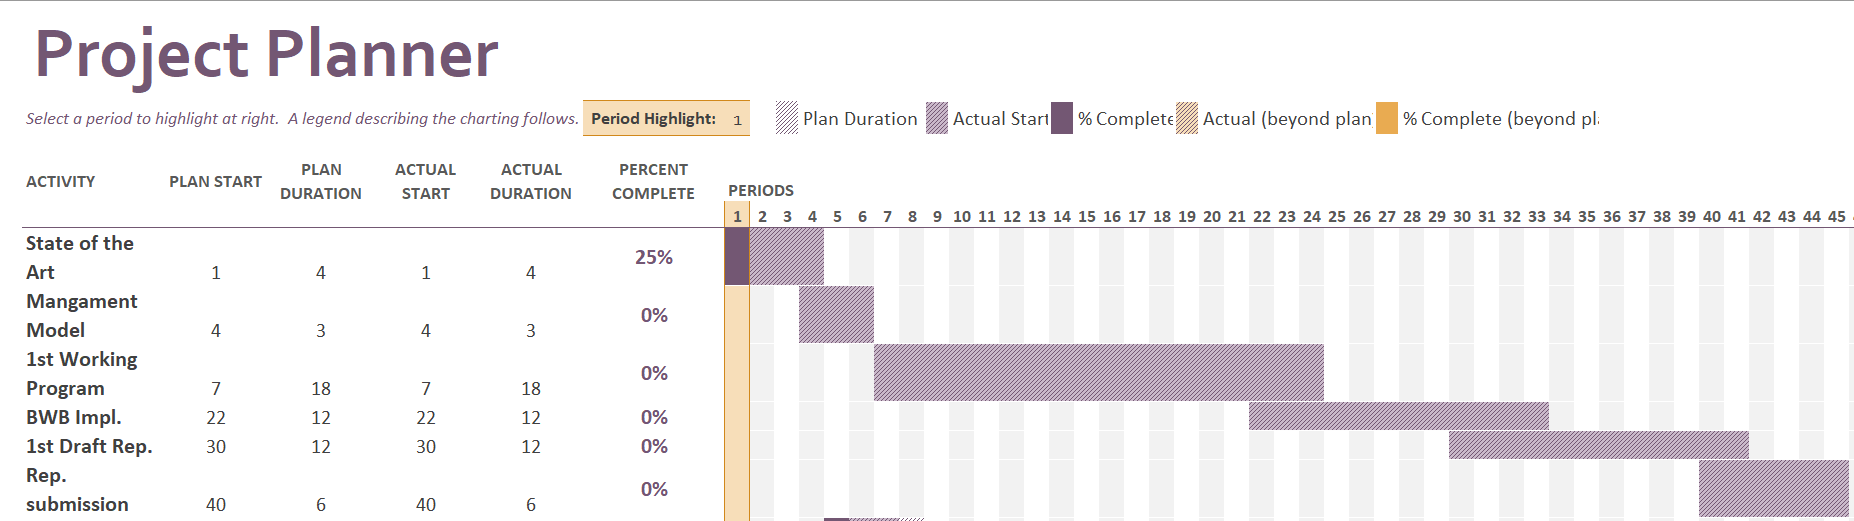
\includegraphics[width=\textwidth]{images/Gantt}
\caption{Gantt chart for the project. A period represents one week, the first week corresponds to the first week of April.}
\label{fig:gantt}
\end{sidewaysfigure}
%%% Local Variables: 
%%% mode: latex
%%% TeX-master: "isae-report-template"
%%% End: 

\section{Write a Multifidelity Aeroelastic Optimization Tool}
%\markboth{l}{Write a Multifidelity Aeroelastic Optimization Too}
\label{sec:task1}
\subsection{Description of work}
The code for the implementation of a Multifidelity Aeroelastic Optimization Tool will be written using the OpenMDAO platform and the corresponding Aerostructures Python package developped at ISAE-SUPAERO. The aforementioned platforms have dedicated libraries to solve optimization problems. A GitHub repository will be created to manage the project. The platform allows version control, branching, collaborative work, among other features. 

Potential flow theory will be used as the Low-Fidelity component of the program through its computational implementation: the panel codes (PANAIR). The structural response will be computed using NASTRAN95, this component is not computationally expensive and thus there is no incentive to simplify it any further. The High-Fidelity component will be a CFD solver. 
\subsection{Technical progress}
No significant advances have occurred during this period, as the state of the art review was underway. 
\subsection{Plan vs achievements}
On time for this task.
\subsection{Changes to the original plan}
No significant changes are needed at this point.
\subsection{Planned work for the next months}
Over the next months, the main objective is to get acquainted with the OpenMDAO platform, the aerostructures package and solve a few sample problems and tutorials. Then, once the strategy for the multifidelity integration is established, the development of the first version of the code will begin. 

\section{Implement the Multifidelity Program to a BWB case}
%\markboth{l}{Write a Multifidelity Aeroelastic Optimization Too}
\label{sec:task2}
\subsection{Description of work}
Once the Multifidelity Optimization Program is fully functional, a BWB study case will be analized using the new tool. There are not many reference cases when it comes to BWB configurations. A conceptual design \cite{Quinlan2019} published by NASA  offers useful data for comparison purposes. The multifidelity optimization of a BWB presented by Bryson \cite{Bryson2019a} is another useful source of reference data. Once the model has been at least partially validated with documental sources, the effect of certain parameters on the final optimized BWB can be explored as well. 

At this point, the focus will not only be on the results themselves, but also in the efficiency of the method. It is interesting to compare its performance to other multifidelity method and single fidelity approaches. Refining the algorithm parameters to improve its efficiency and/or accuracy will be possible during the implementation of the study case. 
\subsection{Technical progress}
No significant advances have occurred during this period.
\subsection{Plan vs achievements}
On time for this task.
\subsection{Changes to the original plan}
No significant changes are needed at this point.
\subsection{Planned work for the next months}
For the moment, the development of this task is out of the scope of this progress report.
%%% Local Variables: 
%%% mode: latex
%%% TeX-master: "isae-report-template"
%%% End: 




\appendix

\bibliographystyle{authoryear-fr}
\bibliography{RPreferences}

\clearpage

\end{document}